\documentclass[UKenglish]{ifimaster}  %% ... or USenglish or norsk or nynorsk
		\usepackage[latin1]{inputenc}         %% ... or utf8 or applemac
		\usepackage[T1]{fontenc,url}
		\usepackage{listings}
		\usepackage{sidecap}
		\urlstyle{sf}
		\usepackage{babel,textcomp,uiosloforside,varioref,graphicx,mathpple}
		\usepackage{tabularx}
		%\usepackage{wrapfig}
		\usepackage{color}
		
\tolerance = 5000 % LaTeX er normalt streng n�r det gjelder linjebrytingen.
\hbadness = \tolerance % Vi vil v�re litt mildere, s�rlig fordi norsk har s�
\pretolerance = 2000 % mange lange sammensatte ord.

\title{Developing Modern Web Applications}
\subtitle{A Comparison of Traditional and Modern Approaches}
\author{Michael K. Gunnulfsen}
\date{Spring 2013}                    %% ... or whenever

%\includeonly{initialization}
\begin{document}
\uiosloforside[kind={Master thesis}]{}

%Include external file. Don't include .tex in the filename
%\maketitle{}

%% NOTES

%% Dynamic HTML is an unofficial term some vendors use to describe effects achievable by combining html css and js based dom manipulation - Engineering book

%% AJAX: Could be worth saying that JS is single threaded and that the UI thread would be frozen while waiting for responds if the AJAX call would be synchronous.
\chapter{Background}     

\section{Introduction}
Web applications has in the last few years seen a dramatic change in both behavior and magnitude. They have grown from being a set simple consistent web pages into highly dynamic, and interactive applications with rich user interfaces. Previously, interactive behavior in web sites were usually performed by Java applets and Flash applications \cite{spa2} that could run inside the browser. But as JavaScript engines and web browsers has become significantly powerful, such behavior is  not only feasible, but increasingly popular to implement with pure JavaScript. Together with this shift towards highly interactive web applications, the user behavior is at the same time increasingly becoming more social. Users makes up the main data content of web applications by socially interacting with each other and adding content to the pages. This chapter focuses on the trends in applications that can be found on the Internet; commonly named as Web 2.0, and the technologies that is commonly used to implement such applications. The chapter begins with a short history of the world wide web, then a discussion of how the web has changed from being simple and static web documents, into dynamic web applications.  Later, we present an overview of the key attributes and common user behavior that is found in modern web applications. Finally an overview of the software architectures and technologies that are commonly used to implement such applications will be given. This background material will be the foundation of the study that has been done in this thesis.


\section{From Web Sites to Web Apps}

\subsection{History of The World Wide Web}
The World Wide Web (www) was first introduced by Sir Tim Berners Lee at the CERN research laboratory in 1989 \cite{firstweb}. He laid out a proposal for a way of managing information on the Internet through hypertext, which is the familiar point-and-click navigation system to browse web pages by following links. At this time, Tim Berners Lee had developed all the tools necessary to browse the Internet. This included the HyperText Transfer Protocol (HTTP), which is the protocol used to request and receive web pages. The HyperText Markup Language (HTML), which is a markup language that describes how information is to be structured on a given web page. The first web server that could deliver web pages, and he built a combined web browser and editor that was able to interpret and display HTML pages. By 1993, CERN declared that the World Wide Web would be open for use by anyone \cite{historyWeb}. This same year, the first widely known graphical browser was released under the name Mosaic \cite{mosaic}, which would later become the popular Netscape browser. Later in 1995, Microsoft would release their compelling browser Internet Explorer, leading to the "browser wars" where each one would try and add more features to the web. Unfortunately, new features were often prioritized in favor for bug fixes, leading to unstable and unreliable browser behavior. Example outcomes were the Microsoft's Cascading Style Sheet (CSS)\cite{css}, which is a language that describes how the HTML elements should appear in the browser. And also, Netscape's JavaScript \cite{jsHistory} was developed to add dynamic behavior that could run in the browser. 

\subsection{The Early Days}
In the mid 90's, web sites were mostly \textbf{static}, meaning that the documents received from a web server were exactly the same each time it was requested. This was only natural, as the majority of web sites were pre-generated HTML pages with lots of static content, e.g a company's home page. Later, however the need for user input became apparent as applications like e-commerce would require two-way communication. User input was not part of the first version of HTML (1.0), which led to the development of HTML 2.0. This standard included \textbf{web forms}, which allowed users to enter data and make choices that was sent to the web server. The development of web sites grew into becoming \textbf{dynamic} web pages. This means that the server responds with different content depending on the input received in HTTP requests. To enable this, there has to be a program running in the web browser, that can evaluate the HTTP request, and generate a proper HTML page depending on the request itself, and the application's state. This is called \textit{server-side dynamic page generation} \cite{tanumbaum}. Another common scenario is \textit{client-side dynamic web page generation}, in which a program is sent to the browser, and executed inside the browser. Examples are JavaScript programs that can achieve dynamic behavior without consulting the server, and applets, which are programs that are compiled to machine code on the client's machine and executed inside the browser. Since applets are compiled to machine code, they execute faster then JavaScript, and therefore, such technologies has for long been favored for implementing performance demanding behavior in the browser. Examples are Java applets, Microsofts ActiveX controls, and Flash \cite{flash}. Java applets are executed on the Java Virtual Machine, which is a cross-platform solution and hence portable to "all" execution environments. Therefore Java applets have been a highly popular way of achieving interactive and dynamic behavior in browsers. Examples include browser games, movies and 3D modeling applications. 

\subsubsection{The Problem with Client-side Technologies}
Java applets and Flash had become popular choices for client-side dynamic page generation by the year 2000 \cite{spa2}, and they still exist in many web applications. There are many problems with this approach however. For instance, a plugin is usually required for running such applications inside the browser, and developers need to know an additional programming model In addition, the user interface tend to look different then the rest of the HTML page, and on top of this there has been numerous examples of security violations with the technology itself \cite{tanumbaumSec}. Using JavaScript would be a preferable solution to client-side interactivity, because it doesn't require an additional programming language or run-time environment considering JavaScript is already supported in all browsers. Having one client language is preferable to facilitate a common development model for all web applications. Unfortunately, this technology has also had its issues ever since it was introduced. Partly because of its buggy implementations due to the scurrying development processes in the early browser wars, which has lead to different JavaScript interpreter implementations by the various browser vendors. But also because browsers have not had the ability to execute JavaScript fast enough to enable satisfying dynamic behavior. For this reason, JavaScript has for long been used as an add-on language for HTML to perform simple roll-over effects,  input validation and pop-up windows.  

However, a lot of work has been done to provide a standardization of the JavaScript programming language. And lately, browser vendors like Google \cite{google} and Mozilla \cite{mozilla} has improved the engines that executes JavaScript to enable the execution of performance demanding processing jobs. 

\subsection{Modern Web Applications}
With the increase of performance capacity in modern web browsers, a lot of work has been done to standardize the development of the web apps, such that cross-platform applications can easily be built to support all browsers. Examples include the work on the newest version of HTML (HTML5). This dramatically simplifies the development of dynamic and interactive client-side behavior and media incorporation without the need for additional plugins. Also, the work on improving the JavaScript language has made it the assembly language of the web, and is now one of the most popular programming languages in the world \cite{jsPopularity}. With this trend towards client-side development, the web has seen an expanding growth in web sites with rich user interfaces and lots of interactive behavior. The technologies has enabled developers to build web sites that looks more like desktop applications with a responsive user interface. Such applications are often referred to as \textbf{"web apps"}, where the browser is the main execution platform. 

\subsubsection{The Social Web and Big Data}
In addition to interactivity and responsive behavior, there is another trend that is a increasingly becoming a key factor in modern web apps; namely social interactions. Many modern web apps, and especially those considered typical Web 2.0 applications (REFR) bases the information content on what the users adds to the page. Usually this includes users posting blog posts, comments, images and other sorts of data information. And in addition, the users connect to each other in a "social network".   Popular "pure" social network applications are Facebook, Twitter, Pinterest and Google+ among others. In addition to web apps that serves primarily to connect users, many other types of applications like e-commerce and e-learning adds social networking ability to their web sites as a way to attract more users, and to get better user-data to improve business value (NEED REFERENCE). Examples include Airbnb, Ebay (both e-commerce), and Coursera (e-learning). 

This behavioral trend has become highly popular, especially considering the users accesses the applications not only on their desktop or laptop machines, but also on smart phones, tablets, TVs, game console etc. Many people accesses their favorite social networking sites up to multiple times a day. All in all this results in a high number of simultaneous users accessing the web applicaitons, leading to high network traffic on the servers hosting these apps. The scalability requirements are massive, enforcing software engineers to design for highly scalable, and efficient backend solutions.

Applications that incorporates social networking features and lets users add content naturally leads to large quantities of persisted data. This has led to the term "big data" (NEED REFERENCE) which describes such large data quantity scenarios that requires efficient and extensible database implementations. Many new database management systems has seen its light since the need to persist large data quantities has increases massively the last few years. Such technologies often have in common that they don't follow the traditional relational database structure (I.e SQL), but adopts other less structural approaches. Such databases are named NoSQL (NEED REFERENCE). The reason they don't implement a relational structure like SQL is that this technology has been showed not to scale when distributed over many database servers. This is a severe problem, because the ability to scale over many machines is not only feasible for load balancing, but an absolute requirement when extremely large amounts of data must be persisted. Most NoSQL databases on the other hand, has showed its ability to scale very well over multiple servers, making it a good choice for persistence solutions, especially when web apps are deployed in the cloud. 
 

\section{Web Technologies}
In this section we will discuss the main technologies that are used to build and host modern web applications. First, an introduction will be given on the client-side technologies that executes the web apps, then we will discuss two different  approaches for designing web-app architecture. The first one is rather traditional and has been widely adopted in web-app architecture the century, while the latter is a much more state-of-the-art approach that follows principles in web architecture that has recently gained much attention. Examples of commonly used web servers are Apache Web Server, and Microsoft Internet Information Server.

\subsection{Web and Application Servers}
Also called HTTP server, is a program running on a dedicated server machine, that hosts web content to client users. The client is usually a web browser, but it could also be a web crawler, who often intends to gather information on web pages searching purposes. The web server usually serves static content, like images, videos, stylesheet files etc, and delegates requests for dynamic content to an \textbf{application server}. The application server hosts the web application itself, also called the backend, \footnote{The application's \textbf{backend} is the application-code that runs on the server, in conjunction to the application's \textbf{front-end} which concerns the code that runs in the browser.}, and hides the low level details of HTTP requests. This way the application server can route specific HTTP requests to appropriate handlers in the web application. Application servers usually supports one or more \textbf{web application frameworks}, which simplifies the development of a web application in a specific programming language. Examples are SpringMVC for Java \cite{expertsOneToOne}, Ruby on Rails for Ruby, and Django for Python. 

\subsection{The Web Browser}
Browsers are software applications that requests and displays information on the Internet. The information is usually expressed in HTML pages, but it can also be other types of data for instance images, script files, PDF files, or videos. The way browsers interprets the data is specified by World Wide Web Consortium (W3C), however up until recently, the various browser vendors have usually not conformed to the whole specification but instead developed custom solutions . This has caused many compatibility issues for web developers.   

\subsubsection{High-level structure}
The browser's software stack consists of a set of components that each has individual responsibilities, and cooperates with the work of fetching and displaying web resources. The main components are listed below :
\begin {enumerate}
\item User interface
\item Browser engine
\item Rendering engine
\item Networking
\item JavaScript interpreter
\item UI backend
\item Data persistence
\end{enumerate} 

The rendering engine is a very important part in the process of displaying a resource. Its responsibility is to get the document from the network layer (usually 8-bits at a time), render the document and finally paint the result on the display. The process of rendering the document is showed in figure \vref{fig:render}. Note that this process is iterative and will happen repetitively until the whole HTML page with all its external resources are completely processed. The rendering engine's lifetime is single-threaded and runs in an infinite loop that listens to events. An event might be to calculate a new position of an element, perform painting on new or modified HTML elements or handle a mouse click. However, if multiple external resources has to be fetched through the networking component,  the browser will create multiple threads that will run in parallel to efficiently load content that needs to be contained in the main HTML document. 

\begin{figure}
\begin{center}
\fbox{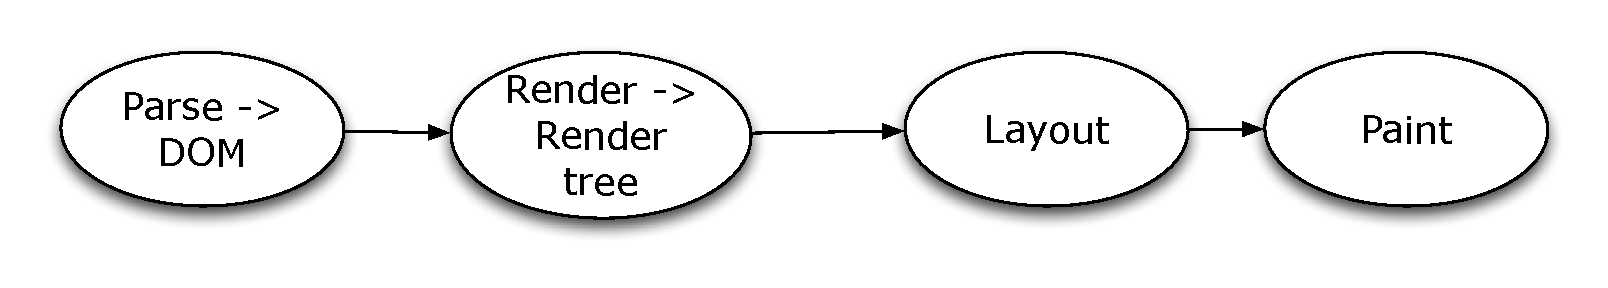
\includegraphics[width=11cm]
{rendering.eps}}
% Kommandoen \fbox tegner en ramme.
\end{center}
\caption{The rendering engine's responsibility}\label{fig:render}
\end{figure}

WebKit and Gecko are two popular rendering engines that implements the rendering process in the figure, however they do differentiate slightly in their internal behavior. WebKit is the engine that runs Chrome and Safari, while Gecko runs Firefox. In this section I have limited the discussion to concern only these platforms, as they are built upon open source solutions and hence have available technical descriptions. The text that follows describes the process of rendering a complete HTML page. This usually happens when the client-browser requests a URL for an HTML page and the browser "refreshes" the page with the new content.

\paragraph{Parsing} 
The rendering of an HTML page starts when the networking layer is instructed to fetch a URL, say \textit{www.google.com}. As the HTML page is fetched, the browser will immediately start fetching all external \textbf{links} that are contained inside the HTML page. This could be links to stylesheet pages, JavaScript pages, images, videos etc. As soon as the initial HTML page is received in the networking layer, the rendering engine will start requesting chunks of data. Then it will start and \textbf{parse} the HTML and stylesheet documents. An important feature of the HTML document's structure is that all the markup elements (tags) are nested in a hierarchical structure. Hence, when the HTML document is parsed, it's tags are laid out in a tree structure, and if an error is found in the page's structure or syntax, an error is thrown. Note however that the HTML parser is "forgiving" in that it will fix errors found in the HTML document.

Whenever the parser hits a script tag it will potentially fetch (if it is external) and execute the script immediately. Unless the tag is marked "deferred" in with case the handling of the script will be postponed until the HTML parsing is done, the parser has to wait until the script is fetched and executed. This is because the script might try to manipulate the DOM tree. To improve performance by avoiding the HTML parser to block while scripts are loaded, scripts can also be marked as "async" in which case the modern browser will to generate a separate thread that possibly fetches and parses the script asynchronously in a separate thread, while the main parser thread can continues with the HTML. Browsers can also create multiple HTTP connections to load external resources in parallel. 
 
 The tree that is generated is called the \textbf{DOM tree}, where each tree element is named a DOM element. When the whole HTML page is completely parsed, the rendering engine will start executing the scripts that are marked   "deferred". When these scripts are finished executing, the browser will generate a \textbf{DOMContentLoaded} event. Finally, if there are any depending scripts that were marked "async" that are still being fetched or executed, and when all external resources are fetched, the window's \textbf{load event} is generated. 

\paragraph{Rendering}
While the DOM tree is being populated, the rendering engine will also start generating the \textbf{Render tree}. This is another tree that is a visual representation of the DOM tree, and in effect decides the style and order for how the DOM elements should be laid out. Every element in the Render tree has a reference to its DOM node, a style, and in addition they know how to layout and paint itself and its children. In effect each render element represents a visual \textbf{rectangle} on the screen. However, it is not necessarily a one-to-one mapping between a DOM element and its render element, because some DOM elements may need multiple rectangles on the screen, and hence have multiple render elements attached to it. The rendering tree is generated from all the styling elements contained in stylesheet documents, styling information in the HTML document, and default styles provided by the browser. While attaching render elements to DOM elements; if the stylesheet is not fully loaded yet, it will save a  "holder" so it can continue later (NOT SURE OF THIS).

\paragraph{Layout}
In the layout process, each render element is given coordinate instructions for where on the screen it will be laid out, and the sizes they will be given. The calculation is performed recursively from the root HTML node to the bottom. Also, the layout process can be global in which the entire rendering tree performs layout calculation, or incremental in which case it uses a dirty bit system; each time a new render element is added or modified it is marked dirty. When an incremental layout process happens it will calculate only the render elements that are marked dirty.

\paragraph{Painting}
The painting process does the actual work of painting the elements on the screen. It does so by iterating through the rendering tree and paints each component. Like the layout calculation, painting can also be done globally on the whole rendering tree, or incrementally. In the latter case, whenever a render element is changed in a way that does not affect the entire tree, the renderer will cause the OS to recognize the changed renderer and hence trigger a \textbf{paint event}.
 
\subsection{JavaScript}
JavaScript is an interpreted programming language primarily built for manipulating web pages. The language was developed at Netscape in 1995, during the time when Netscape and Microsoft were battling for the majority of browser users. The language itself was built in only 10 days, by Brendan Eich. He had instructions to develop a language that would look like Sun's Java, only simpler, interpreted and easy to integrate into web pages, so that it would appeal to non-professional developers. The reason was that at the time, Netscape was built with Java, and the browser-server model was considered a distributed application environment supporting cross-platform development. The only problem was that HTML wasn't sufficient to support complex programming operations, and Java was a rich, and comprehensive language aimed for professional developers \cite{jsin10days}. Hence the need for a hybrid solution. Eich designed the language to follow much of the syntax from the C programming language only simpler and a much more dynamic memory memory management. At the time, a web page's lifetime would usually last from a few seconds to a couple of minuter, and therefore the language had only a simplified concurrency model and me memory management \cite{jsin10days}.

Despite a considerable amount of buggy features in the language and some compatibility issues between the different browsers, JavaScript quickly became a highly popular language for the web. Developers easily create interactive behavior like changing color on a button when a mouse hovers over it, give the user feedback if the input in a textfield i wrong etc. Much of its success was because of its simplicity; there was a low barrier to add JavaScript behavior into web sites. Because there is no compilation process, and no "start function", only independent functions that can easily be written and compiled around in document, unprofessional developers could quickly implement exciting and dynamic features \cite{jsHowGotHere}. On the other hand, for this reason, many professional developers would consider the language of being strictly for amateurs and not suitable for professional developers \cite{UnderstoodJs}.  Its strength however was clearly for small sized applications, as browsers at the time were not able to execute large-scale JavaScript code, and considering that the language at the time was very simple and limited, the development process was simply not feasible. 
 
In an effort to improve the language features of JavaScript, and its browser incompatibilities, a standardization process of JavaScript was given to the European Computer Manufacturers Association (ECMA) in 1996. The language was actually renamed to ECMAScript, allthough most people still refer to it as JavaScript \cite{jsHist}. Unfortunately, as the standardization was being developed, the browser inconsistencies, especially between Netscape and Internet Explorer continued to grow. Many JavaScript frameworks were built as workarounds to the inconsistencies, but most solutions weren't good enough. This led to alternative solutions for interactive client behavior like Flash (REF). 

An important part of JavaScripts history was with the rise of Ajax technologies, which gained much attention about one century after JavaScript was first introduced. Ajax would allow JavaScript code in the browser asynchronously fetch data from the server without having to refresh the current web page. Instead, the requested data would be used to manipulate the web page. This would result in a much more interactive user experience because the browser would neither block while waiting for the request, or re-render and paint the whole DOM tree. Since the introduction to Ajax, JavaScript has increasingly became a highly popular language, and it brought the attention of professional developers. This led to successful framework solutions like JQuery and Prototype (REF), which simplifies the development of complex dynamic behavior and browser incompatibilities.

The increasing popularity of client-side application development with JavaScript has led to powerful JavaScript engines in modern browsers, making memory management and JavaScript interpretation highly effective. In September 2008, Google built the Chrome browser with its V8 JavaScript engine, stating that low performance JavaScript implementations are no longer sufficient. Other browser vendors followed along, and today JavaScript performance is more superior than ever. Still, however there are drawbacks with the language itself. Even though libraries like JQuery and Prototype simplifies the development of interactive and cross-platform web pages, it is easy to end up with a big pile of tangled JavaScript event handlers and unstructured functions. Most of the reason is that the language lacks features like classes, modules and namespaces, which makes it difficult to develop flexible and maintainable large-scale JavaScript applications. However, a lot of work has been done lately to implement quality frameworks that provides comprehensible syntactic sugaring for the language. These frameworks use the nice concepts of the JavaScript language like inheritance and closures to enable a highly flexible and structured development environment. All this has led to a massive amount of large-scale JavaScript web applications where much of the backend code has been moved to the client tier, implemented in pure JavaScript.


\subsection{Client-server Interaction Schemes}
There are multiple ways the browser can communicate with the web server. In this thesis, we mainly adhere to two different ways ways: synchronous client-initiated requests, and asynchronous browser initiated requests. These are both client-pull based, however there are other push-based alternatives like Comet, or WebSockets, where the client and server maintains an open connection, and the server notifies the client of changes. The communication schemes all use HTTP .

\subsubsection{Synchronous}
In a synchronous HTTP request, the client-browser asks the server for data, in which the browser will wait for the server to respond. The request is normally trigged by the user who writes a URL in the browser and presses enter, or an HTML form that is submitted. This could be a button that is pressed inside an HTML form tag, the enter key is pressed inside a text field that is contained in a form tag, or a link that is clicked on a given page. The server usually responds with a new HTML page that is sent to the browser, in which case the browser would start a complete rendering process to build a new DOM tree, and paint it on the screen.  

\subsubsection{Asynchronous}
In asynchronous HTTP requests, the client-browser sends a request to the server and continues to execute without waiting for the server to respond. When the server has completed handling the request, it will send the respond to the browser, which is then notified and will handle the result. Usually in this communication scheme, the result is not a complete HTML page, but rather a more fine-grained data object. In this case the browser would perhaps manipulate the DOM tree to alter the page content in correspondence with the result that came from the server. The browser does not have to reload the page, since the browser's data structures (DOM/rendering trees) does not have to be re-built. The client user is usually unaware of the request, because the browser doesn't block while the communication happens.

The most popular form of asynchronous communication is with Ajax technologies. This lets the application programmer use JavaScript to send HTTP requests to the user. When the server-response is received, the browser will initiate and event, in which the developer would have created an event-handler that parses the result, and performs some action based on the result. The result is normally sent as XML, or JSON data. These are both common data formats used in HTTP transmissions. 

One potential drawback with Ajax is that not all browsers supports JavaScript. Examples are some smartphone devices or PDA devices. Also, some old browser implementations would not let Ajax requests send the browser to a new state. This means that if the user hits the back button after an Ajax request has been performed, the browser would go back to the last full-page reload that was accessed, instead of going back to the page as it was right before the Ajax request. Last, pages that are generated using Ajax is not automatically picked up by web crawlers, because most web crawlers does not access JavaScript code. This means that content generated by Ajax would normally don't show up in public web searches (NEED REF). 

\subsection{HTTP Sessions}
The HTTP protocol is stateless, meaning a new connection must be set up for each client-server request. Therefore, to be able to maintain state throughout a "session", \footnote{An HTTP-session is a semi-permanent communication dialogue that exists for two communicating entities (here, the client and the server). A session normally has a time-out value, such that when the time runs out, the session ends. } state information has to be persisted somehow. The state information itself is data that has to be maintained between multiple pages in the application. Examples are shopping cart information in an e-commerce site, flight booking details, or authentication credentials. Imagine the user having to identify himself for each request he sends to the server. This can be avoided if state information is persisted and being referenced for each request. 

There are a couple of ways to handle session state. It can be persisted on the client, on the server, or inside the messages sent between the client and server. As for server generated sessions, an implementation is usually provided by the web application framework that hosts the particular application. In this case, the server generates a session-object that will contain session data. This object can be kept in-memory, in the database or stored in flat files. To identify the session object when a request comes into the server, some web frameworks choose to put a unique id in the browser's cookies, or if cookies are not supported by the browser, inside every URL in the web application. The session identifier is then included in every HTTP request the user sends to the server. An example is given in figure \vref{fig:httpsession}. Note that the session object can, and often is used as a cache for data that the given user would access often. That is if the session object lives in the server's memory and not in the database. This avoids having to fetch the same data from the database needless times.

Session state can also be maintained inside the messages themselves, that are sent between the client and server. This could be to place data inside hidden fields in HTML forms, store the data in cookies, or store the data in the URL. However, this approach is not very flexible, as the data has to be manually coded into all the places in the HTML pages where requests are sent to the server, plus that the data size is limited, as is the data format.

The third alternative is to store session state in the client's browser. This works in the same way as the server-side approach, in that a session object is stored in browser memory or some external database controlled by the browser. The advantage of this approach is that no session identifier has to be included in the HTTP requests sent to the server, since everything is managed by the client. If the session is to be stored in the browser's memory, the browser has to support HTML5, which provides a programming interface (API) for communicating with an in-memory database in the browser.  

\subsection{Representational State Transfer}
In web applications, each individual HTTP request is is handled by a particular function that resides in the application's backend. Modern web applications often follows a design pattern named Representational State Transfer, or simply REST. {\cite{engineering} This pattern states that all HTTP URL's must reference a particular resource on the backend, by using one of the four supported HTTP operations Get, Post, Put, or Delete. This way, every URL offered by the web application are self-contained in that it contains all the necessary information needed to satisfy a request. Resources are identified by a URI, which uniquely identifies a resource, and one of the four HTTP methods that should be performed on the resource. Applications that follows this pattern are named RESTful applications. A common use case for RESTful applications is to offer the self-contained URL's publicly to clients other then just the application's own front-end, like other third party applications that wishes to use the applications REST services. Further, the REST pattern states that each REST request is stateless, hence adhering to the nature of HTTP which is stateless. That means that REST requests should not depend on an ongoing session in order to generate proper results.

\subsection{JSON}
JSON is a text based data format that is based on a subset of the JavaScript programming language. It is easy for both humans to read, and machines to parse, and has a similar syntax to many of the programming language based on C. The data structure fits well as a transmission format in web applications, because it is both simple and light weight, easy to modify and is supported by many programming languages. The format itself is very simple, and the datatypes offered are limited to numbers, strings, arrays, objects (key-value pairs) and booleans. An example of a JSON object representing a guitarist is showed below:
	\begin{lstlisting}
	{
		"username": "Paul Swayer",
		"age":21,
		"country": "Norway"
		"guitars": 
		[
			"Gibson Les Paul",
			"Fender Stratocaster"
		]
	}
	\end{lstlisting}
This object contains two string key-value pairs, one integer value, and one array consisting of two simple string values. Notice how the object itself is made up of key-value pairs. RESTfull applications often use JSON as a transmission format. For instance a JSON object can be sent with a PUT request, so that the REST receiver will update the object with the content in the JSON object. Also, in a REST get request, the receiver can return a REST object to the client.

The closest alternative to JSON is XML, which is another transmission format often used on the web, and especially with REST communication. However, its syntax is a bit more verbous, and requires more processing to marshall because of its markup tags. On the other hand XML lets one add more restrictions to the data then with JSON.


\subsection{Template Rendering}
In dynamic web pages, when an HTTP request comes in for a particular HTML page, the server has to prepare and populate the HTML page with proper content before the completed page is sent back. Normally the server inspects the HTTP request that comes in by looking at the HTTP request headers, the content of the HTTP body, and the session identifier and the URL. Given the information provided in the request, the server will perform some action, and probably fetch data from the database. This data is to be placed in the HTML page that will be returned to the client.

One way to generate an HTML page that contains the newly generated content, is to generate the HTML directly in code as Strings, and send the result back to the client. However this approach is messy, difficult to maintain, and the developer has to know the programming language that generates creates the HTML strings. In other words, not a preferable solution for web designers who only knows HTML. The preferable approach is to use a templating system. A template system consists template files, which are HTML pages that contains special markup code that refers to and can operate on the data from the application. The operations supported are usually limited to simple loops and conditional expressions, just enough to facilitate the injection of dynamic data without confusing front-end designers. The template system also has a template rendering engine that takes a template file, the data to populate the file, and produces an HTML page. This way, when a client request comes in, the server will generate some data, probably from the database or in-memory cache, create an object that is filled this data, and send the object together with the proper template page into the template rendering engine. The resulting HTML page is sent back to the client. 

Template rendering can also happen on the client. This would be performed by JavaScript code inside the HTML page. This is done by adding special syntax in the HTML page that is recognized by a rendering engine, and ignored by the browser. When some HTML page is to be rendered, the JavaScript rendering engine (which lives in the client) would be called with an HTML page and a data object as input, and it would return with the same HTML page altered with with the new content from the data object. Unlike server-side page rendering, there are no special file type for template files. They are just HTML pages with special syntax that is ignored by the browser when the HTML page is rendered. Hence server-side template rendering generates a new file given a template file, while client-side template rendering modifies an existing HTML file. 

\subsection{Databases}
Storing persistent information is an essential part of web applications. The content that is offered must be able to be saved, retrieved, deleted and modified in an efficient and flexible manner. Databases, and especially relational databases has since the beginning of web application history been the most popular form of storing persistent data \cite{engineering}. Other alternatives have been used like flat-file storage (where the content is stored as plain text or binary data) or XML- or object databases, but ever since relational database management systems arose back in the early 1970s, it has been a highly popular form of data persistence. The reason is that it provides \textbf{durability}, which in the context of data persistency means that once the data is stored, it is guaranteed to exist even if machines holding the data crashes. Another reason for relational databases's popularity is that it stores information in a structured format, which often fits the structured data formats that are manipulated by the web applications. However, as the extent of information being persisted in modern web applications has become incredibly large, other types of database technologies has lately entered the marked. These are commonly referred to as NoSQL databases.

\subsubsection{CRUD operations}
In web application terminology, one often use the word CRUD to refer to the four essential  database operations; \textit{Create}, \textit{Read}, \textit{Update} and \textit{Delete}. These are operations performed by the web application, on the data that needs to be persisted. When a CRUD operation is executed, it is the applications responsibility to convert the data into a format that fits the database's technology, and vice-versa. This process is called marshaling, or serializing. One example is when the application is to save a new object in the database. In this case, a \textit{Create} operation will be performed where the application will transform the object from whatever programming language syntax the object is currently described in, into a structure that fits the given databases' syntax. The application will send this transformed (marshaled) object to the database, which is now able to parse the object and save it to its storage structure.   

\subsubsection{Relational databases}
Relational database management systems (\textit{RDBMS}) is a storage system based on a formalism known as the relational model. The formalism is based on structure and relationships, where the data  entities are stored into \textbf{tables} that contains a set of \textbf{attributes} that describes the table. The tables can be related to each other to form groupings. RDBMS's stores a collection of tables, where each data entity is represented as a \textbf{row} in a specific table, and each column in a row represents an attribute for that entity. The most popular form of manipulating data in a RDBMS is SQL (Structured Query Language) \cite{sql}. This is a query language used to insert and manipulate data in a relational database. There are popular dialects of the language, generated by database vendors like Oracle's SQL, Microsoft's MS SQL  and the open source product PostgreSQL. 

\subsubsection{NoSQL}
	NoSQL is a broad class of various database management systems who all have in common that they don't share the relational structure from normal SQL databases. The main potential for noSQL databases is to perform operations on massive amounts of data that is not structured or connected in complex relationships. Very often this applies to web 2.0 applications, because much of the information in such applications can be persisted as simple key-value data, where the values can be arrays of key-value data. A typical example is users that has arrays of blog posts, and blog posts has arrays of comments, in which case the users and blogposts would be identified by a name (key). There are many different classifications of noSQL databases, which vary in the way they structure the data. An overview of the most common used noSQL categories is summaries in the following list:
\begin{description}
  \item[Key/value store] \hfill \\
	Is a simple database store where data is identified by a key, and the data itself can be any datatypes usually supported by the implementing programming language. The structure is schema-less, meaning it doesn't provide complex structures with foreign key constraints. It is also highly efficient as the database is often implemented as a HashMap. Examples are Dynomite, Voldemort, Redis etc.
  \item[Document-oriented databases] \hfill \\
  Is a datastore that is based on documents that contains unstructured content. However there is some variation in the way the different database implementations choose to define the formats of the documents, but it is assumed that each document encapsulates some logically associated data in a predefined format. An interesting property with these databases is that performance is often not the main goal, but rather programming satisfaction. As many of these are implemented in JavaScript and offers querying semantics and data structures based on JavaScript objects, it is really easy and flexible to perform database operations on them. Examples include CouchDB and MongoDB. 
  \item[Column-oriented databases] \hfill \\
  Is a database system where data is organized as columns, as opposed to row-oriented databases such as SQL based databases. In this scenario, every  value that would usually be in a row gets its own instance in a column together with its belonging ID. As such, it is very efficient to perform range queries over a big amount of column data. Examples are Cassandra and Google Big Table (although these are not pure column-oriented, but rather a hybrid). 
	 \ldots
\end{description}

\section{Summary}

\chapter {Design Alternatives for Modern Web Applications}
\section{Introduction}
So far we have discussed the behavioral trends in modern web applications, and some common technologies that enables such applications. We saw that modern web applications are often very interactive with rich user interfaces, and that these web sites looks and performs like native desktop applications with graphical user interfaces. In addition there is often a requirement for a high number of simultaneous users, and a lot of data is being stored and manipulated. In this chapter, we look at the various technologies that are commonly used to design and build such interactive and scalable software applications. This concerns the overall architecture, both seen from a hardware and software perspective. 

As the behavioral requirements for web applications has increasingly changed the last years, so has the application's software architectures. The traditional web application has in the last decade followed a three-layered architecture where all the logic happens on the server. This is called a fat-server architecture, where HTML pages are rendered on the server and handed to the browser every time the client sends a request. Lately however, there has been an increasing interest in moving much of the applications logic to the client, and abandoning the server-side page rendering in favor for client-side page rendering for dynamic HTML content. This is called a thick client architecture. \footnote{The thick client architecture is not a new idea; thick client architectures has been around for many years, where programs are sent from the server and executed in the client. Often this would be online games, calculators, or other user-interactive applications. However, these applications depend on a specific program that is compiled and executed on the client, in other words, not traditional web pages that uses common browser-supported technologies.} Still however, a lot of applications follows the traditional approach, as many developers and application owners are skeptical to the fat-client model. This architecture implies heavy use of JavaScript, which has since its beginning had a lot of opposition, and there are still many browsers that does not fully support JavaScript behavior. 

The main purpose of this chapter is to outline the differences between the traditional web-app architecture, and modern web-app architecture, in the purpose of building modern, interactive and scalable web 2.0 applications. The chapter is divided into two main sections, one for each architecture,  where each section will discuss some common architectural principles, and give some concrete examples from real-world scenarios. For simplicity purposes, we will refer to the traditional approach as \textbf{Architecture 1.0}, while the latter approach will be referred to as \textbf{Architecture 2.0}.

\section{Traditional Web Application Architecture}
Going back approximately 15 years, web applications where often built with CGI technology using tools like Perl and ColdFusion \cite{webstart} . With the CGI technology, a web server accepts URLs that are delegated to an appropriate CGI program. A process is started on the server, and the CGI program executes the given request, which results in an HTML page that is sent back to the client. This solution however, was not very scalable considering each request would trigger a new process on the server. Gradually, as the web got more users and the applications became more complex, new web framework technologies came along. Examples are PHP, J2EE, Ruby on Rails and Microsoft's .NET \cite{topframeworks}. For many years, developers have been building web applications with these technologies, where all of the application's business operations are executed on the server. This implies that the backend implementation has many responsibilities, and the front-end is simply a thin client that doesn't need to do much processing. This is only logical, as backend implementations runs on powerful web servers, and client devices has up until recent years not been able to perform demanding processing jobs. 

In an HTTP request, the backend application receives requests (often named an \textbf{action}) from a client which is handled by a \textbf{request handler}. The handler performs validation of the input data, executes the necessary business logic, and if necessary, manipulates the database. To be able to serve multiple simultaneous users, the application server often generates a separate thread for each incoming request. At the end of the handler's execution sequence, the application prepares an HTML page that it sends back to the client. The client tier refers to the front-end code that runs in the client's browser. It consists of an HTML and zero or more CSS files. The modern web application proposed in this thesis requires a lot of interactive behavior which is usually best solved with  JavaScript. Other popular alternatives to JavaScript are for example Flash, Microsoft Silverlight, or ActiveX. However, these all have in common that most browsers don't support them out of the box, meaning a plugin has to be downloaded and installed in order to use any one of them. Also, these technologies tend to provide their own graphical user interface, so that when they are integrated into the web app, they tend to look different then the web app's own "style". 

The HTML file contains just the necessary JavaScript code to enhance the user experience. The script code is either embedded in the HTML file inside \textit{script} tags, or it is referenced as external JavaScript files that must be fetched by the browser. The JavaScript code is often a collection of \textbf{event-handlers}, which are independent functions registered to be notified when a given event happens in the browser. Examples of events is when a mouse is clicked that will start an animation, the mouse is hovering over an image, a button is clicked that will open a small pop-up window, or some text is entered that needs quick validation. The event-handler will look at the current state of the web page, execute some necessary JavaScript routine, possibly making an Ajax request to the server to get some data, then manipulate the browser's DOM tree to update the page. Note that the JavaScript event handlers are only used for small-sized user events that needs quick results. User actions that leads to bigger changes, like URL- or form requests are not handled by JavaScript but are normal HTTP requests sent directly to the server, leading to a new HTML page sent back to the client. 

%When the browser receives the data from the server, it will do nothing more then simply display the %data, and not perform any additional business logic. This is a best-practise  usage scheme that is %recommended by most web developers \cite{separateBusiness}. and is referred to as a thin client %model.	 

% flash er n� bakt inn i chrome og ie 10.
% Flash og java er vanligvis brukt til multimedia shit



%%% Need form validation both on client side and server in case user has shut off client side JS. 
% He could submit invalid data, and abuse the server impl. We can have client side validation for efficiency reason in addition to it. 

%% Script tag in head blocks browser 
%% Script in bottom, can let page render so user sees stuff while page loads
%% Script tags blocks, therefore asynchronous module loading.
	
%The server maintains state for each user, most often by using an HTTP-session implementation. This %way, the first time the client uses the app, the server creates a session object that is used to %remember what the user has done.

%	The backend implementation in a \textit{web app}, is the code that runs
%on the server. This is often deployd
%	in an application server. The backend code is invoked by a web server
%application, that sits
%	and listens for incoming http connections. In the traditional approach,
%the user executes an
%	http request each time it triggers an html form, or requests a url
%either in the address bar or through
%	an html link tag. An html form is a component that wraps other input
%components like a button, textfield, date picker etc.
%	In other words, each time the user initiates an action, an http request
%is sent to the server. 
%	In this case, the server would respond with a complete html page that
%the browser renders so the user can see it on the screen. Also, it is not
%	the case that the server sends the whole web page in one http response
%packet. Each reference to other resources that are embedded in the html page (which
%could for instance be a movie reference, css style sheet reference, or javascript source file
%reference) are fetched in a separate http request. In some cases the response from
%the server could be an http redirect,
%	which is an instruction to tell the client to make a
%	request for a new page. This would in effect require a
%	(minimum) number of 4 client-server interactions! Considering that this
%process	is synchronous (because the client has to wait until the server has sent
%the html page back), it might lead to tedious waiting time for the client
%user.
%	
%	\subsubsection{Ajax}
%	Obviously, this interaction scheme is not always ideal for interactive
%web applications, especially if only a minor part of the web page is changed in
%the http request. Hence, having to send a complete html page each time the user
%performs an
%	action is in many cases a waste of network traffic. This has lead to
%another popular
%	client-server technology called Ajax \cite{ajx}. In this interaction
%scheme the browser
%	would only ask the server for a specific web resource. This could for
%instance be a blog
%	post or comment represented in a markup language like XML \cite{xml}.
%When the browser receives this resource
%	from the server, it would embed it into the already rendered web page.
%This process happens 
%	asynchronusly, and the web page is not refreshed upon completion. In
%result, there user wouldn't
%	have to wait for some data transfer to finish (since it happens
%asynchronously behind the scenes),
%	and the received data is much more fine-grained.
%	
%	\subsection{Client state}
%	Since http is stateless, the server has to maintain state between a
%given client's requests in order to avoid having to ask for user credentials all
%the time. 
%Now, there are a couple of ways to solve this, and it is usually implemented in
%web application frameworks.
%Some choose to put a unique id in cookies, and some choose to add an id to each url,
%or inside hidden fields in html forms. The most common choice however, is to use
%so-called html session objects. This is implemented as a token identifier that
%is stored either in a cookie or in the url (if cookies are not supported by the
%browser). This is called a session object, and is 
%included in every http request the user sends to the server. Hence, the server
%has to maintain a session
%object in memory for every user that is accessing the page at any given time. An
%example is given in figure \vref{fig:httpsession}. The session object is often used a cache for data object that the given user would access often. This avoids having to fetch the same data from the database needless times.
%
%\begin{figure}
%
%\fbox{\includegraphics[width=\textwidth,height=\textheight,keepaspectratio] 
%{images/httpsession.jpg}}
%\caption{A HTTP request with a seesion identifier in the cookie}
%\label{fig:httpsession}
%\end{figure} 

%\subsection{Server-side page rendering} 	
%	In dynamic web pages, when an http request comes in from the user,
%	the server has to have a way of dynamically updating the given html page
%	that is requested with new data. This might be data recently fetched from a database, or maybe some data
%	that is currently stored in the servers memory. The html page is often
%	generated on the server by using a so-called templating engine. This 
%	component will take as input a map of data variables, and a so-called
%	template file. The template file is a source file written in a domain
%	specific language. This language extends html with a set of predefined tags.
%	The tags represents basic programming concepts like variables, loops, and
%condition statements.
%	When the templating engine executes the rendering job, it 
%	transforms the template file and the data map into a complete html page
%	that it sends back to the client. 
	

	
\subsection{The Three-Layered Architecture}		
A classical way of separating concerns in a web application is to divide the whole system into three different software layers. This is called a three-layered architecture, and is composed of a Presentation layer, domain layer, and a data source layer \ref{brown}. These layers reside on the backend of the application. The front-end has little responsibility in this architecture, as its only task is to display the result that is produced on the backend. The layers are designed to be very loose coupled. This is done by avoiding that a module in one layer depends on a concrete implementation in a lower layer. Instead, they depend on abstractions (interfaces) which can easily be swapped out \ref{dip}. The abstractions are not hard-coded into the layers, but are "injected" through function arguments so that the same function can be called again if one wants to change the type of a dependency. The benefits from having individual implementation details encapsulated in different layers, is that it is very easy to modify one layer without harming another. And in addition, layers can be reused by other software modules. For instance, the data source layer could be re-used by another module that also wants to use the database, but does not want to have to go through a domain, or presentation layer. 		
		
\paragraph{The presentation layer} is responsible for displaying information to the end-user by accepting HTTP requests, and return prepared HTML pages. The presentation layer is the main entry point on the backend, where URL requests are received and handled by a dedicated action handler. Such a handler is often called a \textbf{controller}, which is a dedicated function that is called by the application server, to handle the URL request. Often the URL request goes through a number of filters before control is handed to the controller. Filters can have different objectives like authentication, marshaling of different web formats into an object in the programming language that is used , error handling or input validation. Also, the presentation layer would check the URL for a session identifier in the request's cookie, or the URL itself. If there is one, the session identifier is referencing a session object that is in already residing on the server's main memory, or it is fetched from a database. The presentation layer might validate the data parameters that are found in the HTTP request and verify that the user (identified by the session object) is allowed to perform the action it requests. After request are passed the filters, the appropriate controller function is called. The controller function usually has little responsibility, other then to delegate to the right business function in the domain layer, possibly together with some data objects found in the session object, and parameters given in the request URL. 

When the business function returns back to the controller, it looks at the result to determine which view to return back to the end user. The view might be an HTML page, a page written in a template language, or another data-format like XML or JSON. The latter two formats are most often used if the request is an Ajax request, in which case the client just wants some data with no markup formatting added to it. Then the controller handles the resulting object to a marshaller which transfers the result object into either XML or JSON. If the view to return is a template file, the controller will handle the execution on to the rendering engine which compiles the template file together possibly with a data object that is being used to populate the page during rendering. The data object might be the result of the business operation (for instance some data that was fetched from the database), or some data that is stored in session object (which may have been modified during this process). In which case the controller would send this data into the rendering engine together with the view itself. The result of the rendering process is a new HTML file that is sent back to the client user. It is also possible for the controller to send multiple template files into the rendering engine in order to produce one single HTML file as result. This comes in hand if the various pages on the web app contains multiple repeating HTML fragments. Typically this might be a navigation bar or a  footer. In this case these reoccurring HTML pieces could be implemented in separate template files, and reused in the different pages.



\paragraph{The domain layer} is responsible for executing the business functions that are supported in the web application. These are the functions that makes up the core services of the application. The domain layer should be built with an emphasis on flexible and coherent code so that the business rules can easily be extended and modified. To enable this one should design with proper design patterns and
techniques like test-driven development \cite{beck}. It is in the domain layer one can find the domain objects (or business objects) that acts as the representation of the core entities that exists in an application. The business operations in the domain layer uses the domain object, by performing various  actions on them. Examples are calculating the total price for an order of books, registering a new friendship between two users, or searching for recommended movies for a currently logged in user. 
There are multiple ways of organizing how the business processes are implemented in a domain layer. For example in the domain model design pattern \cite{poea}, the domain objects knows how to perform business operations on themselves. While in the transaction script pattern \cite{poea}, the
business logic is encapsulated in separate functions that operates on the domain objects. The business operations (or transaction scripts) are independent procedures that has a one-to-one
mapping with the actions supported in the presentation layer (e.g the web site). The domain objects
are completely stripped from any business logic functions, they merely contain the data attributes as field values. The domain objects are usually encapsulated in the first-order citizen types used by application's programming language. For instance in Java or Ruby, a book would be represented in its own Book class, a movie would have a Movie class, an order would have an Order class etc. 
	
\paragraph{The data source layer} is responsible for communicating with other systems, such as databases, messaging systems, external web services, the filesystem etc. In the context of persistency, this layer is responsible for converting the in-memory objects into the proper storage representation, and vice-versa. For instance translating a SQL table into a Java object. The data source layer has to connect to the database, handle database transactions and close database connections. Usually this is handled by the web application framework, so the data source layer only has to worry about how to perform operations on the database. As with the domain layer, there are two popular patterns for structuring the data source layer. One is with the active record pattern \cite{poea}, in which case each domain object would know how to perform CRUD operations on themselves. Another approach is the data mapper pattern \cite{poea} where there is one separate class for each domain object, that is responsible for performing the marshaling of the given domain object. For instance, if there is a class \textit{Person} in Java, it could have a reference to a mapper class called \textit{PersonMapper}. This class could have 4 functions, one for each CRUD operation. These function would know how to communicate with the database, execute SQL queries, and transform a Person object to a SQL table and vice-versa. The data mapper pattern separates the persistence code out of the domain objects, but adds more classes to the system. The active record pattern has a tendency to grow big in size, if the domain objects has to support a large amount of complex database operations. 
	
There are also frameworks that hides the complexity converting between database entities, to in-memory objects. These are called object-relational mapping (ORM) tools, and are framework injected into the application that creates an in-memory version of the database. They often provide caching mechanisms to avoid using the database as much as possible, and they allow the programmer not to worry about the details in the database implementation, as this is handled by the ORM tool. In many cases this could lead to less code in the data source layer. \cite{lessCode} Examples are Hibernate \cite{hibernate} for java, MyBatis\cite{mybatis} for Microsoft .net and Java,
and LINQ \cite{linq} for Microsoft's .NET. It is important to point out that even though these frameworks hide the complexity of object-relational mapping, it does have some pitfalls. Many developers argue that by using ORM-tools you loose the ability to exploit the full features of a
database management system. \cite{ormlame}This includes the ability to do customized database tuning, and take advantage of special data types that are supported by specific vendors. Plus, the fact that an ORM-tool does indeed hide the object-relational mapping code, makes it hard to do debugging and write complex and efficient queries. At last, there might be some performance overhead provided by the code that is generated by the ORM implementation.
	
	
\subsection{The Front-End}
In the previous section we discussed the backend implementation of a traditional web app. The backend covers the majority of the application's source code, as it is responsible for almost everything, except displaying the HTML page. This is done on the client, and it is referred to as the front-end implementation. The front-end consists of the set of HTML pages, CSS style sheets and script files that makes up the user interface of the application. An important intent with the thin-client architecture, is that the client browser does not have to perform any heavy script computation or business logic operation, because everything is prepared by the backend.

Typically, when a client first accesses a given web app, the request goes to the server which responds with an HTML file. This file includes CSS stylesheets and JavaScript source files, either as references to external sources, or embedded inside the HTML. Also, the HTTP response usually includes a request for the browser to form a cookie with a given session identifier. The browser will immediately start rendering the HTML file. When the DOM tree is built and ready, the browser will generate a DOM-ready event. This event triggers the execution of some minor JavaScript initialization code. This code is responsible for setting up event listeners and connecting  appropriate event handlers to them. When the whole page is fully loaded with all external sources  fetched, the browser triggers the onLoad event, and the page is ready to be used.

Typical actions the user performs when navigating around on the page are either handled by HTML input forms or hyperlinks, or a JavaScript event handler that is registered with an event listener to execute an interactive request. If a user action is meant to result in a simple and interactive operation (like a displaying a pop-up window or an animation effect on a mouse-hover event), the event is usually handled by a JavaScript event handler which executes the operation quickly in the browser. Everything else is performed by an HTML form or a hyperlink. Every HTML form or hyperlink has a one-to-one mapping with a corresponding controller handler on the server. This mapping is represented in the form of a URL. When a form is executed or hyperlink is followed, an HTTP request is sent to the server. The request holds parameters that are meant for the controller handler. These are received in the controller handler on the server as normal function parameters, that the controller will use to execute the action. The parameters were created in the HTML form, or in the hyperlinks, embedded in the URL itself. The controller handler on the server executes the action, and creates a new HTML page that is sent back to the browser. The browser will  then again repeat the initial scenario where the new page goes through the rendering process, external sources are fetched, and new JavaScript event listeners are initialized. 

				
\subsection{Platform environment}
Another aspect of the classical three-layered architecture is application tiering \footnote{Application layering is a term that divides the code into separate logical software layers. Application tiering on the other hand, is another logical separation often associated with where these "tiers" are physically deployed. For instance a three-tiered web application could have its presentation tier on the web server, logical tier on the application server, and persistence tier on a database server.}. A web application is often divided into three tiers; the presentation tier, the logic tier, and the persistence tier. A benefit by having this separation of physical tiers, is that the tiers can be re-used and distributed in a parallel computing environment to gain performance benefits. However, it does bring communication overhead when data is transferred between tiers, plus that synchronization can become a challenge. 

The web server hosts the presentation tier which communicates with client users through HTTP. The web server listens on port 80, which is the port number used for HTTP. The HTTP request is forwarded directly to the appropriate code on an application server. The application that runs on the application server communicates with the persistence tier that is usually hosted on one or more database servers. During the development process of an application, all the tiers are normally deployd on the same machine. This means that the developer has an app- and web server running on the localhost IP address on his personal development computer. In a bigger production environment, it is normal to distribute the tiers into separate physical server machines. Also, for large scale deployments, each tier can be distributed to multiple servers. In this case, a load balancer is used to delegate requests to available servers, and manage the communication. This is showed in figure \vref{fig:ntier2}. Each server is hosted on a separate machine in a so-called shared nothing manner, meaning the servers on each tier doesn't communicate with each other. This makes it easy to add more servers on demand without any synchronization difficulties. Note that when the persistence tier is composed of a relational database management system, a shared-nothing architecture is difficult to implement, due to the nature of the relational model \cite{dataCloud}. This makes it difficult to do horizontal scaling with relational database systems. However, with applications that mainly performs read-tasks, one approach is to have a master-slave architecture, where one master node makes the writes, while other slave nodes offers read operations. Each time a master updates a table, the update is propagated to the slaves.
				
	\begin{figure}
	\begin{center}
	\fbox{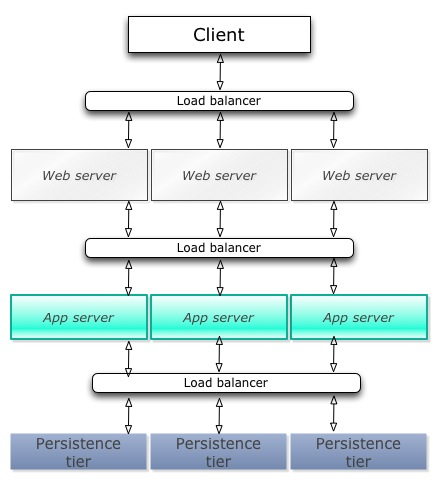
\includegraphics[width=10cm] {images/ntier2.jpg}}
	% Kommandoen \fbox tegner en ramme.
	\end{center}
	\caption{A distributed production architecture}\label{fig:ntier2}
	\end{figure}
				
				
\subsection{Examples of traditional web architectures}
In this section we will look at two examples of some common, traditional three-layered web application architectures. The examples use web application frameworks that is made for different programming languages. The purpose is to propose a set of popular web architectures, that will be used as a base to determine the architecture we use to design the first prototype in this project. 
				
\paragraph{MVC with Ruby on Rails}. The Rails framework for Ruby has become a highly popular backend technology for web applications with big commercial users like Twitter and Git-Hub \cite{railsPop}. The framework is built around the MVC design pattern \cite{mvc}. In a Rails application, the controllers acts as thin classes that simply delegates business logic to the Models. The model classes are built around the domain model design pattern, meaning they will perform business operations directly on themselves. The model objects also knows how to do database mapping, by communicating with for instance a relational database. The view layer consists of template files written in a template language like HAML\cite{haml} or ERB. These templates can reference Ruby model objects, and are rendered into HTML files on the server before they are sent to the client's browser. 
				
Ruby on Rails encourages developers to use RESTful URL's so that these are automatically mapped to specific controller actions. The Rails developer can define the set of (RESTful) URL's that the application will support, and the framework will in return create controller handlers for each URL with appropriate model objects that are being referred to in the URL. This principle is called \textit{convention over configuration}, because the framework sees the RESTful convention in the URL where a model is referenced by a URI, and the operation is defined by either one of the HTTP methods GET, PUT, POST or DELETE. The controller actions usually performs CRUD operations on the appropriate Model object that is referenced in the URL. This is again accomplished automatically in Rails by using the convention over configuration principle. This is applied to the data source layer, where database tables are automatically created from a Model class. Table names and attributes are created by default, determined by the names and types in the Model's ruby class. For instance, if a Model class is named \emph{Movie}, Rails will create a database table called \emph{Movies} that
has all the fields that exists in the Movie class. The data source layer is built with the active record pattern, so that every Model knows how to perform database operations on itself. The Rails framework makes it possible to build web applications quickly with a small amount of code, because Rails generates many of the basic structures and operations previously mentioned. In addition,
the loose coupling that results from the MVC pattern makes the application easy to distribute in a cloud environment, because if designed properly, each tier has a shared-nothing relationship. They are independent, and can be cloned and deployed on separate servers, as depicted in figure \vref{fig:ntier2}. This is much of the reason that Rails has gained a lot of popularity lately in the web
application industry \cite{someREF}% NEED REF!

\paragraph{Front Controller with SpringMVC}
Just like with Rails, SpringMVC is also built around the MVC pattern, however the controller part is built using the \textbf{Front controller} pattern. This pattern works by having a single entrance point for all the HTTP requests, that sits and consolidates actions to various routines that is to be executed for each URL. This can be seen in figure \vref{fig:springmvc}.
				\begin{figure}
	\begin{center}
	\fbox{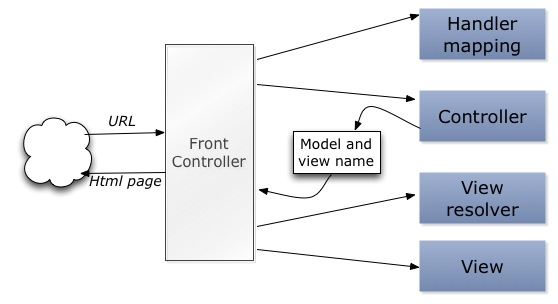
\includegraphics[width=10cm] {images/springmvc.jpg}}
	% Kommandoen \fbox tegner en ramme.
	\end{center}
	\caption{A request flow with spring MVC}\label{fig:springmvc}
	\end{figure}
	
When a request comes in, the front controller will ask a \textbf{handler mapper} to get a reference to a specific \textbf{controller handler} based on the URL. In addition the handler mapper performs a set of pre- and post processing procedures, like validating the input from an HTML form, or marshaling an XML object to a Java class. The front controller then receives a reference to the controller handler, and the front controller will further delegate the request to this handler. The controller handler is usually responsible for performing some business operation implemented by the application programmer. When the business operation completes, the controller handler populates a \emph{Model} object with necessary data that is to be displayed in the \textbf{view}. The model object is a simple key-value data structure that lets the developer easily reference its data from the view file. The controller function also returns the name for the view that is to be rendered together with the Model object. The \textbf{view} is a template file written in a template language like JSP or Velocity. It is the \textbf{view resolver} that maps a logical view name (e.g "homePageView") to a physical view name (e.g "/WEB-INF/views/homePageView.jsp"). Finally the view and the Model object is rendered to HTML and send back to the client. 
	
With Spring comes a great implementation of an inversion of control container (IOC)\cite {ioc}. Inversion Of Control is a programming methodology where the concrete types of object references are not know at compile time, because the references are instantiated and populated  by an assembler at run time. This avoids having tight couplings between classes, and promotes a flexible codebase. The IOC container is a module that is responsible for creating objects, populate their references  to other objects, and manage their complete lifecycle. The container is fully configurable, which makes it easy to decide how the classes are instantiated. This could be by lazy loading (the object isn't instantiated until accessed), a singleton (only one instance of a class is allowed to be created), one instance for each session, or one for each HTTP request. The IOC container provides a component based structure for the application by following the dependency inversion principle \cite {dip}. This principle states that object should not depend upon details, but rather abstractions. This means that the spring IOC container will inject concrete objects into components (which are interface references and not references to concrete classes) at run time. This enhances the decoupling of classes, because they have the freedom to decide the types of their owning references at run time, instead of compile time. The container works as an object factory, and makes it easy to add new components to the application while at the same time hiding the implementation details of the added behavior. An alternative way of composing the application with external modules is to use the service locator design pattern \cite {j2ee}, which is a common approach taken in Java EE based applications. Dhrubojoyoti Kayal \cite{Kayal} shows how the service locator pattern can be implemented in Java Spring applications. However considering Spring already has an IOC implementation, it might lead to a lot of boilerplate code to assemble components using the Service locator pattern. 
			
Another nice feature with Spring is that it has built in support for both relational- and noSQL database management implementations, as well as transaction management. On top of this it supports annotation-based declarations making it easy to customize features using java annotations \footnote{Annotations: A way to add meta-data information in the source code. Metadata is often provided by configuration files, but annotations enables this information to be populated directly on the java declarations in the class files. An example is to use annotations to define how each variable in a java class is represented as a SQL column.} This conforms to the convention over configuration principle, which leads to simple and quick web application development. 
			
A typical domain layer in a spring application is built with the service layer pattern \cite{serviceLayer}. In the service layer pattern, the business operations are categorized into logical abstractions called \textbf{services}, where each abstraction is hidden behind a facade \cite{facade}. A facade is an interface that contains simple access methods to a more complex set of data structures, like complex business operations or database access methods.  Hence, each service encapsulates complex business operations and communicates with lower layer data source functions. There are also \textbf{domain objects} that represents the main data entities in the application. These domain object are simple java classes with no logical functions, only private data attributes with accessor methods. The service classes uses the domain objects, and communicates with the data source layer. The service classes are also responsible for handling transaction management, so that if a transaction fails, the service classes knows how to handle it. When performing transactions, the service classes delegates to the data source layer which would know how to communicate with the database and perform object-relational mapping. This could be done by implementing a customized object-relation mapping scheme, for instance by implementing the data mapper pattern described earlier, or by using an ORM tool like Hibernate or JPA. The latter case is similar to the active record pattern used in Ruby on Rails. 


\section{Modern Web Application Architecture}
The motivation for proposing a reference model for modern web-app architecture has its roots in an architectural shift that started around 2008-2009.\cite{hales64} At this time, a new form of client-server interation scheme was emerging away from the traditional hyperlink/form-oriented request-response scheme, where each time the client interacts with the application, a request is sent to the server in which a new HTML page is created and sent back, and the browser has to reload the entire page. In addition, AJAX technology had been around for a long time, which usually was being used when some data is needed from the server for some minor interactive behavior. Building applications completely based on JavaScrip with Ajax for server communication was possible, however most developers had acknowledged the fact that such front-end oriented architectures doesn't scale in terms of code flexibility; it often ends up as piles of spaghetti code. This is partly because of web developers' relationship to JavaScript; as stated earlier, JavaScript has had its buggy features and lots of browser incompatibility problems since its early beginnings. Also, many professional developers has a misunderstood relationship to the language; they are not aware of JavaScript's key language features like object-orientation including prototypal inheritance, and functional- and dynamic programming facilities, having closures and a dynamic typing system. Also, developing large-scale JavaScript applications is difficult, because the language lacks constructs that facilitates flexible and modular code. It is possible to create namespaces and class-based structures with JavaScript, but it requires a lot of effort because it needs to be built from the ground up in every application. However, this was only until recent years, because a lot of work has been done to build frameworks that neatly solves these problems. 

%(TODO: skriv om n�r ECMAScript ble standardisert i kmap1), 
The architectural shift began in 2010, when browser's capabilities to execute JavaScript increased tremendously. This was by the time when Google launched its Chrome browser with the powerful V8 JavaScript engine, and the compelling browsers followed along with similar JavaScript capabilities. Also, The JavaScript language itself has started to get much more endorsement from the web community with the standardization of ECMAScript, and Google's provenly working large-scale JavaScript applications like Gmail, Google Maps and also Node. This has led to many new experimental web architectures that takes a distance from the thick server model, and where application state is gradually moving from the server and into the client. However, not only is the application state gradually being moved to client, but also the application logic. This means that the core application moves from the backend to the client, leaving the backend being a simple and agnostic storage center for persisting the domain data in the application. Not only is this feasibly, but it's becoming increasingly popular. 

Handling state on the client means that the one-to-one mappings between user interactions and controller handlers on the server are gone. Form requests and hyperlinks aren't sent directly to the backend, but instead handled on the front end. The only time the server is contacted is when data is needed to be fetched or manipulated in the database, authentication of users, or the browser needs to fetch static content like for instance images, movies, stylesheets or script files. The front-end tier has taken over most of the responsibilities that used to be done on the server, which now involves:
\begin{itemize}
\item{} Routing between pages
\item{} Render views into HTML
\item{} Sessions and state handling
\item{} Business logic operations
\item{} Input validation
\item{} Language translation of content
\item{} Deciding what to store in the database and when
\end{itemize}
 
Now, there are variations in how many of these responsibilities that are performed mainly by the client. Input validation for instance usually needs to be done on the server in addition to client-side validation, in case the user manages to contact the server directly without going through the front- end. Also, some applications might prefer to let the server be involved in routing between pages (ref to airbnb), and perform some of the page rendering (ref to twitter). There are many good reasons for moving the backend responsibility to the client's front end. Some key advantages are:
	
	\begin{itemize}
	\item Centralization of the application's codebase, since much of the application logic, and the dynamic presentation logic is now located in the same place, and implemented in the same programming language
	 \item Less load on the server because more processing is moved to the client
	\item Facilitates smart front-end techniques like lazy loading of HTML- and script files, because JavaScript techniques can be used to only fetch HTML and script files when needed.
	\item The presentation logic and application logic lies much closer together in terms of source code. This facilitate tight cooperation and integration and be built with familiar design patterns in only one language: JavaScript. Such tight cooperation where hard to implement with the traditional approach, because it required tight cooperation between a template language (e.g JSP), JavaScript, and a backend language like Java.  
	\item Enables the server to offer a more general-purpose interface to the outside world. It no longed serves to deliver content to one particular client, but also other types of clients like third-party applications
\end{itemize}

The responsibility of the backend is mainly to manage the database. It's interface is still exposed as controller handlers, however these are not customized for particular HTML form requests or hyperlinks that leads to a new HTML page. Instead, the backend exposes an \textbf{API} for interacting with the application's domain data. This API contains a set of public functions where each function is identified by a specific URL. Each URL refers to a domain entity in the application, and an operation that the server is to perform on the domain object. Note that this operation is usually not a complex business operation, but merely a single database operation. The operations offered by the backend API are commonly expressed using merely HTTP methods. Hence, the server API is a RESTfull service that adheres to the principles in the REST design pattern. Now, instead of creating and returning a complete HTML page upon each client request, the server would return a more fine-grained data object represented in a uniform data format like XML or JSON. This is a much more general-purpose solution, because external clients like mobile applications and other third party applications can now use the service offered by the application, because the service will no longer only respond with entire HTML pages, but a fine-grained format that is easier to manipulate and use as desired. This is often referred to as a service-oriented architecture \footnote{Many service-oriented architecture experts does not consider REST as a part of the SOA-paradigm, mainly because it is resource-oriented rather then service oriented}. 


	
Another interesting aspect of modern web application development is the evolution of JavaScript development environments. Not only has JavaScript been judged for being a language with many limitations, but it has also lacked proper development tools  like editors and debuggers, and frameworks for syntactic sugaring. Even though JavaScript is, and has always been a highly popular language for web applications, it has mostly been used as a tool to add dynamic behavior, input validation and simple Ajax calls to the server. With the increasing interest for large-scale JavaScript client applications, a huge amount of frameworks and language variations have been built. This includes:
\begin{itemize}
\item{} A huge amount of frameworks for structuring and organizing JavaScript code. \footnote{There is an project (REF) on www.Github.com(REF) where open source developers are implementing the same web application with different JavaScript frameworks to help developers choose a proper code organization framework for their web apps. (REF) }
\item{} Programming languages that compiles to JavaScript, to facilitate the development of large-scale JavaScript applications with a language that is more similar to traditional languages like Java or Ruby. Examples are Coffescript (ref) and clojure script(ref).
\item{} Syntactic sugaring frameworks that provides utility functions for operating on various JavaScript data structures, doing mathematical operations, or fixing browser compatibility issues.
\item{} Rendering engines for the front end, built to render HTML code with data objects.
\end{itemize}

	
Together with this thick-client approach one has also seen a sudden interest in alternatives to the traditional relational database. With the increasing popularity of applications being deployed and run in the cloud, there is a need to be able to distribute an application's database over many servers. Now it so happens that normal relational database structures has showed to have transactional challenges, and lacks scalability when distributed in the cloud \cite{dataCloud}. These issues, together with the demand for extreme high performance, has led to the development of new persistence technologies that are specifically designed to work well in a cloud environment. The so-called noSQL paradigm is a common term for classification of database technologies that does not belong to the family of relational databases. These technologies has gained massive popularity in the last couple of years, because is has showed to deliver excellent performance and scalability in cloud environments. In addition, many of the noSQL technologies are built to fit nicely together with JavaScript, which makes it easier for JavaScript based applications to manage the database. 

In the next few sections, I will dig further into the ideas and technologies that typically makes up the modern web-app architecture.
	
\subsection{Thick client tier}
In the traditional architecture, almost all of the business logic is implemented on the server, and the only code that is executed on the client is the JavaScript functions necessary for generating dynamic behavior in the browser. The idea in this proposition however, is to move the application's logic to the front-end. The business logic involves the domain objects and the operations that are performed on them, data validation, language translation of data, and communication with third-party API's. Instead of programming this logic in a proper backend language like Java or Ruby, this is  implemented in JavaScript, or a language that compiles to JavaScript, like CoffeeScript or Clojure script. The front-end source code is located on the web server as publicly available static assets. All the source code has its root in the main HTML file which is sent the client the first time he uses the app. The HTML file contains references to the JavaScript source file(s) that makes up the front-end application, such that the browser automatically fetches these when the main HTML page is being rendered. Typically the JavaScript code is separated over multiple source files. Also, the HTML page will have references to external JavaScript framework files that are not developed by the application programmer, but is used inside the app's own JavaScript code.
	
	The JavaScript code can either be sent to the client all at once when the web application is first accessed, or it can be lazily fetched. The latter means that the client will only ask for the necessary part of the code, when it needs it. This requires the source code to be split into separate code files so they can be sent individually from the server. This might be a performance benefit in case the whole JavaScript codebase is very big. A pitfall however might be that very many small JavaScript files are required at the same time. In some cases the TCP connection overhead might lead to a performance bottleneck because the browser usually creates a new TCP connection every time the browser requests something from the server. Sending all the scripts (and HTML and CSS files)  on startup gives the advantage of being able to gather all the JavaScript logic into one single file that can be extensively minimized and compressed. In this case, no further source files are needed to be fetched from the server, but the initial load time might be overwhelming. It is also possible to do a compromise, where the programmer gathers the most commonly used scripts into one compressed file that is sent initially, and then lets the client fetch the rest only when it is first needed. 
	
\subsection{Single-page Application Architecture}
One essential advantage of the thick client architecture is that server requests can now be limited. In the traditional approach, each user interaction with the page leads to a server requests that result in a new page, and the browser has to reload the whole page. This causes a disruption in the user experience. With the modern approach, the request goes straight to JavaScript event handlers. This way, the client stays on the same page during the whole session, requiring no new page reloads. If for instance a link in the navigation bar that leads to a different "section" in the app is requested, everything is done in the browser by manipulating the DOM tree so that the page moves to a new state. This leads could to a much more fluid user experience, because server requests can be avoided, and the browser does not have to reload the entire page. This principle is commonly referred to as a Single-page app (REF).  

If the front-end needs to synchronize data with the database it will send an asynchronous to the server. This could for instance be to save some data, or get some new data that needs to be displayed on the page. The client can also save data in the browser's memory, such that the more domain objects stored in the browser's JavaScript memory heap, the less requests has to be sent to the server. Depending on the application, write, update and delete operations will always sooner or later have to lead to a server request. In applications that requires all updated data to be available as close to real-time as possible, the operations has to be directly written to the database, in effect work as a write-through cache. In applications where this requirement is more relaxed, the front-end can choose to perform the server persistence at a later, more appropriate time. For web 2.0 applications, the former is often wanted, because users usually want to be see the latest updated data at all time. 
		
\subsection{REST API's and JSON}
The thick client model avoids letting the user communicate synchronously with the server. Instead, the JavaScript application that runs in the browser is responsible for knowing when it needs to communicate with the server. This would be whenever some domain objects that are not already in the browser's heap are requested, or some domain object must be persisted to the database. The requests to the server are exclusively done through a RESTful API. This means that all domain objects that are to be offered by the server, must be accessed through one of the HTTP methods \textit{GET, POST, PUT, or DELETE}. An example of a RESTful API that offers functions for persisting a Shredder object is showed in table below. A shredder is a guitarist in the web-app prototype that has been created in this thesis.
	
	\begin{center}
	\begin{tabularx}
	{\linewidth}{ |X|X|X| }
	    \hline
	    \textbf{Method} & \textbf{URL}  & \textbf{Description} \\ \hline
	    Get & www.shredhub.com/ shredder/1234 & Get shredder with id 1234 \\ \hline
	    Post & www.shredhub.com/ shredder/ ?name=Jude Swayer & Add shredder with name Jude Swayer  \\ \hline
	    Put & www.shredhub.com/ shredder/ 1234?country=Sweden & Update shredder with id = 1234 set country = Sweden \\ \hline
	    Delete & www.shredhub.com/ shredder/1234 & Delete shredder with id 1234 \\ \hline
	    \end{tabularx}
	    \end{center}
	    
	The server would respond with the domain objects in JSON format, instead of a complete HTML file. In effect, the return value is much more fine-grained. Also, the API is very consistent, because it adheres to a common interaction scheme, namely the HTTP functions Get, Post Put, and Delete. This creates a familiar and easily-to-understand server API. Many modern web application frameworks like Ruby on Rails, Spring MVC and Django are built based on the principles of REST, and will automatically create RESTfull controller functions based on the application's domain objects. This programming interface works really well with the thick client model, because now the client tier can be 100\% responsible of maintaining the application's state, and use the backend as a simple persistence API to store and deliver the domain objects. Hence, the backend is just a simple service that knows nothing about how to visualize the domain objects in HTML, leaving this responsible to the client tier. 
	
Modern REST API's very often use JSON as the transmission format. The reason is that it fits well into the programming model both on the front end and backend, because considering that the front end code is implemented in JavaScript, and JSON is part of the JavaScript language, it is very appropriate to use JSON as a transmission format because no marshaling has to be done on the client. At the same time on the backend, it is so that some of the noSQL technologies uses JSON objects, or JSON-similar syntax for persisting data. Hence we get a common transmission format that can be used across the whole software layer stack. 


	
\subsection{Modular JavaScript}
A modular codebase is made up of highly decoupled, encapsulated pieces of coherent features that are implemented in separate modules. A codebase that consists of loosely coupled modules,  facilities a flexible and maintainable system, because the codebase contains less dependencies\cite{henrik}. This makes it easier to change one part of the system without harming any other.  
	As previously stated, the JavaScript programming language does not have module features built into the language. This means that it is up to the developers themselves to develop some sort of module framework. Various design patterns have been proposed to establish standard ways of developing modules, like the module and sandbox pattern \cite{jspatterns}. A lot of work has been done to provide open solutions for JavaScript developers to build modular JavaScript code, the two most famous being AMD (Asynchronous Module Definition) and CommonJS. Having the JavaScript code separated into modules means that these modules can be split into separate source files. That is what facilitates the lazy loading of JavaScript files previously mentioned. The modules can even depend on HTML files, so that whenever a JavaScript module is loaded, the HTML page will be loaded as well, and will be available as a text string inside the JavaScript module. With this feature, we can now state that the JavaScript modules are the first-class citizens in the application and hence decide which and when a given HTML page is to be displayed in the browser. This is an important difference from Architecture 1.0 where the HTML pages where the first-class citizens, and the JavaScript code was just embedded inside the HTML. 
	
	The AMD principle was made to have a better alternative to loading scripts then the traditional group of \textit{<script>} tags embedded in HTML files. AMD brings an API that facilitates the separation of JavaScript into modules and defines the modules' dependencies to other modules. These dependencies are asynchronously loaded into the module, which avoids browsers having to block while waiting for synchronous module loading. the AMD API comes with two functions: require() and define(). Define() is used to encapsulate a JavaScript module while at the same time define the other module it depends on. The require() is used to asynchronously load modules into a function, in which the function will not be called until all the modules are loaded and ready to be used inside the function.

	%CommonJS is another module format meant to encapsulate JavaScrip into separate modules. %[MORE ON THIS].

	\subsection{Client side page-rendering}
	In Architecture 1.0, every HTML page is completely rendered on the server and never changed after the page is sent to the clients. In Architecture 2.0 however, this idea is completely abandoned. HTML pages are rendered "on the fly" with JavaScript code that is executed on the client side. The HTML pages contains templating markup that is detected by a JavaScript rendering engine. Whenever a new HTML page is to be loaded, or embedded into the current HTML page, a certain JavaScript function will be called. This function is responsible for asking the rendering engine to take an HTML page together with a set of JavaScript objects that represents the data that is to be displayed in the page, and finally return the HTML page with the JavaScript data rendered inside it. 
	As previously mentioned, the AMD model makes is possible to have JavaScript modules that depends on HTML files. This facilitates a nice programming model, because if the HTML pages are also separated into small, independent modules, then these modules can be stitched together to form complete HTML pages. For example, a JavaScript module might depend on a small HTML module, and when the JavaScript module is loaded, it can render the HTML module and insert it in the current HTML page. As such, HTML modules can be reused, removed or swapped out from the current HTML page by the JavaScript renderer. This enables a highly flexible way of altering contents of the HTML page, and also to easily glue together reusable front end solutions. 
		
	\subsection{Client state}
	Another part of Architecture 2.0 is how the state is being kept between requests. The major goal of Architecture 2.0 is to move much of the application logic from the server to the client. Hence, being able to keep the state client side is of high priority. In this architecture, we propose a solution to this by using HTML 5's Web Storage. The HTML 5 web storage is a standardization made by W3C that defines how to store structured data in the browser between page requests. It is supported by all browsers, except Internet Explorer 7 and earlier versions. HTML 5 web storage contains two storage containers: local storage and session storage. The difference is that local storage is being persisted even when the browser is closed, and it has no expiration date. The session storage is only kept in the browsers memory until the session is over, which means either if the user closes the tab or the browser. The storage enables developers to store lots of more data then what it supported with cookies. As an example, Internet Explorer 8 allows for session storage up to 10 mega bytes, while a cookie is limited to 4 kilo bytes. The session storage is consists of a key-value data structure that is accessed by a simple JavaScript API.
	
	The session implementation is built by letting a JavaScript object be created when the web application is first accessed by the client user. The object is populated with account information for the user, and can be extended with data values that is appropriate to be cached in the browser. Each time the client tier changes state or receives some state information from the server, it can be persisted in the session object. Hence the server does not have to maintain a session object in memory for each user that is currently logged in to the web application.
				
	\section{Summary} 
In this chapter we have proposed two very different web architectures. A short comparison of these two can be seen in the table below. The table sums up the major differences between the two architectures, where each row is concerning similar application issues. 

\begin{center}
	\begin{tabularx}
	{\linewidth}{ |X|X | }
	    \hline
	    \textbf{Architecture 1.0} & \textbf{Architecture 2.0} \\ \hline
	    Server-side page rendering & Client-side page rendering \\ \hline
	    Application logic runs on server (thick server) & Application logic runs in browser (thick client)  \\ \hline
	    Session state stored on server & Session state stored in browser \\ \hline
	    Form-based interaction with complete html pages returned & RESTfull ajax requests for JSON objects and asynchronous module loading \\ \hline
	    Relational database system & Document-oriented database based on key-value semantics \\ \hline
	    \end{tabularx}
	    \end{center}


Architecture 1.0 had a thin client model with all the business
logic performed on the server. The server's job was to perform the business
operations, execute database operations and render a view that is sent back to
the client. I argued that having a decoupled n-tier architecture could make it
possible to distribute each tier in the cloud, but the problem with having a
relational database could lead to that being a bottleneck. The latter approach
had a thick client model where most of the logic was performed in the client's
browser, primarily using the server for database operations. This could lead
to a structured and loosely coupled front-end implementation, as well as a
reduced amount of data sent back and forth between the client and server. The
RESTfull architecture, together with asynchronous HTML/JavaScript loading
can make it possible to limit the data that is sent back
back from and to the server, since the only time a complete html page request is required is
the first time the page is accessed. However the first HTTP request might turn
in to being a very big data package, since a lot of� javascript has to be sent to the client.
This could in worst case could lead to a very slow initialization time.
 Also since the data format is cross-platform, other external
clients like third party users and mobile applications can use the service
offered by the application. Finally, the noSQL database characteristics seems to
be more suitable in a cloud environment, because it is possible to shard the
database tier with in a shared-nothing manner. It also provides programmer
friendliness due to its simple syntax. 			



\section{Summary}


\bibliographystyle{plain}  
\begin{thebibliography}{9}

\bibitem{hales64}
Wesley Hales,
\emph{HTML5 and JavaScript Web Apps (Page 64)},
O�Reilly Media, Inc, 2013

\bibitem{spa2}
Michael S. Mikowski, Josh C. Powell,
\emph{Single Page Web Applications (Page 2-3)},
Manning Publications Co, 2013

\bibitem{firstweb}
\emph{The website of the world's first-ever web server},
http://info.cern.ch/,
CERN 2008

\bibitem{historyWeb}
W3C,
\emph{A Little History of the World Wide Web},
http://www.w3.org/History.html

\bibitem{mosaic}
\emph{NCSA Mosaic -- September 10, 1993 Demo},
http://www.totic.org/nscp/demodoc/demo.html

\bibitem{css}
\emph{CSS},
http://www.w3.org/Style/CSS/

\bibitem{jsHistory}
\emph{A Brief History Of JavaScript},
http://javascript.about.com/od/reference/a/history.htm

\bibitem{tanumbaum}
Andre S.Tanumbaum, David J. Wetherall,
\emph{Computer Networks (page 691)},
Pearson Education Inc. 2011

\bibitem{tanumbaumSec}
Andre S.Tanumbaum, David J. Wetherall,
\emph{Computer Networks (page 875-877)},
Pearson Education Inc. 2011

\bibitem{flash}
\emph{Adobe Flash runtimes},
http://www.adobe.com/products/flashruntimes.html

\bibitem{mozilla}
\emph{Mozilla},
http://www.mozilla.org/en-US/

\bibitem{google}
\emph{Google},
https://www.google.com/intl/us/about/

\bibitem{jsPopularity}
\emph{JavaScript Leads The Pack As Most Popular Programming Language}
http://www.webpronews.com/javascript-leads-the-pack-as-most-popular-programming-language-2012-09

\bibitem{jsin10days}
Charles Severance,
\emph{JavaScript: Designing a Language in 10 Days},
Computer (IEEE Computer Society) 45 (2): 7�8.

\bibitem{jsHowGotHere}
\emph{JavaScript: How Did We Get Here},
http://www.oreillynet.com/pub/a/javascript/2001/04/06/js\_history.html

\bibitem{jsHist}
\emph{A brief History of JavaScript},
http://javascript.about.com/od/reference/a/history.htm

\bibitem{UnderstoodJs}
Douglas Crockford,
\emph{The World's Most Misunderstood Programming Language},
http://www.crockford.com/javascript/javascript.html

\bibitem{rest}
Roy T. Fielding,
\emph{Architectural Styles and the Design of Network-based Software Architectures},
University Of California, Irvine, 2000

\bibitem{engineering}
David Patterson, Armando Fox,
\emph{Engineering Long-Lasting Software: An Agile Approach Using SaaS and Cloud Computing},
Strawberry Canyon LLC, August 24, 2012

\bibitem{lessCode}
Douglas Barry, Torsten Stanienda,
\emph{Transparent persistence vs. JDBC call-level interfaces},
http://www.service-architecture.com/object-relational-mapping/articles/transparent\_persistence\_vs\_jdbc\_call-level\_interface.html,
1998

\bibitem{ormlame}
Craig Walls,
\emph{Spring in Action},
Manning Publications Co, 2011

\bibitem{railsPop}
http://rubyonrails.org/applications


\end{thebibliography}

\end{document}